% Provenance (never printed): see sources/outline_sources.md (Year 3: gravitational
% potential, spherical harmonics, J2, reference ellipsoid, geoid, satellite gravimetry,
% flexure of the lithosphere). Brief: sources/book5/BRIEFS.md, ch. 3. Curves from
% figdata/bachelor-3/hydrostatic_figure.py, ice_mass.py (IMBIE 2021), flexure.py.
% Exercise and problem values in the Book 5 scratch calculator calc/ch03.py.
\chapter{Gravedad y figura de la Tierra}\label{ch:b3:gravity-geodesy}

Dos satélites vuelan uno detrás de otro alrededor de la Tierra, a una altitud de más
de \qty{500}{km} y a unos \qty{220}{km} uno de otro, y miden sin cesar la distancia
que los separa, con una precisión de un micrómetro.
% ledger: geod5:grace, geod5:grace-ranging
Cuando sobrevuelan una zona donde la masa está concentrada, el satélite delantero
es atraído primero hacia delante y la separación se abre; después el trasero es atraído
a su vez y la separación se cierra. A partir de esas variaciones minúsculas, mes tras mes desde 2002,
se ha cartografiado el campo gravitatorio de la Tierra en su evolución: el agua almacenada en
las cuencas fluviales sube y baja con las estaciones, y los grandes casquetes de hielo de
Groenlandia y la Antártida pierden masa año tras año. La gravedad pesa lo que el ojo
no puede ver. Este capítulo construye el campo gravitatorio de un planeta en rotación a partir de su
potencial, obtiene de él el achatamiento y el momento de inercia, sigue sus
anomalías hasta la órbita, y después se ocupa de uno de los efectos que la gravedad revela en
la superficie: la flexión de la litosfera bajo el peso de un volcán.

\begin{recall}
La ley de gravitación de Newton, la energía potencial gravitatoria y la
fuerza centrífuga en un sistema de referencia en rotación se estudian en los libros de física; los momentos de
inercia de un sólido y los polinomios de Legendre $P_2(x) = (3x^2 - 1)/2$ se estudian en
los volúmenes universitarios de física y matemáticas; el módulo de Young $E$ y
el coeficiente de Poisson $\nu$ en el volumen de tercer año de los libros de física. La geodesia y el
achatamiento $f = (a - b)/a$ de un elipsoide de semiejes $a > b$ se vieron en el
año 10. Isostasia, compensación de Airy, gravedad normal, geoide, altura del geoide y
anomalías de la gravedad se definieron en el volumen de primer año, en su
capítulo sobre isostasia y anomalías de la gravedad.
\end{recall}

\section{El geopotencial}

En un planeta en rotación, un cuerpo en reposo siente la atracción de la masa del planeta
y, en el sistema de referencia que gira con él, la fuerza centrífuga. Ambas derivan de un
potencial.

\begin{definition}[Geopotencial]\label{def:b3:gravity-geodesy:geopotential}
El \emph{geopotencial}\index{geopotencial} es la energía potencial por unidad de
masa, en el sistema de referencia que gira con la Tierra a la velocidad angular $\omega$, de
la gravitación y la fuerza centrífuga en conjunto:
\[
  W(\mathbf r) = V(\mathbf r) + \Phi(\mathbf r),\qquad
  V(\mathbf r) = -G\int_{\text{Tierra}}\frac{\mathrm dm'}{|\mathbf r - \mathbf r'|},\qquad
  \Phi(\mathbf r) = -\tfrac12\omega^2 s^2,
\]
donde $s$ es la distancia al eje de rotación. La gravedad es
$\mathbf g = -\nabla W$, y las superficies $W = \text{cte}$ son sus
superficies de nivel: en cada punto, la gravedad es normal a ellas.
\end{definition}

Una plomada cuelga según $-\nabla W$, y el agua en reposo se acomoda sobre una
superficie de nivel. Un planeta fluido en rotación adopta, por tanto, la forma de una de sus
superficies de nivel: el potencial centrífugo, más profundo en el ecuador, abulta el
ecuador y aplana los polos.

\begin{omfigure}
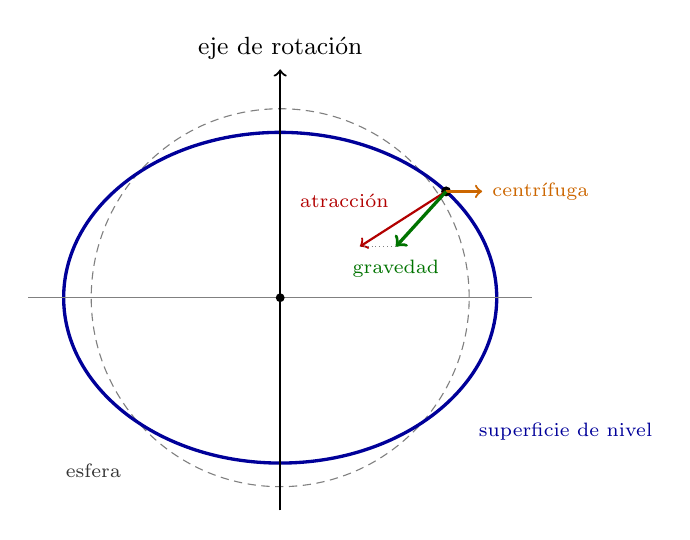
\begin{tikzpicture}[font=\small, x=1cm, y=1cm]
\draw[gray, densely dashed] (0,0) circle (2.4);
\draw[very thick, blue!60!black] (0,0) ellipse (2.75 and 2.1);
\draw[->, thick] (0,-2.7) -- (0,2.9) node[above] {eje de rotación};
\draw[gray] (-3.2,0) -- (3.2,0);
\fill (0,0) circle (1.6pt);
% a point at latitude 40 deg (parameter) on the ellipse; the attraction points at
% the centre, the centrifugal force is horizontal, and their sum is drawn along the
% inward normal of the ellipse: lengths solved so that the sum is normal (calc/ch03_fig.py)
\coordinate (P) at (2.107,1.350);
\fill (P) circle (1.8pt);
\draw[->, thick, red!70!black] (P) -- (1.012,0.650);
\node[font=\scriptsize, red!70!black, anchor=south east] at (1.50,1.02) {atracción};
\draw[->, thick, orange!80!black] (P) -- (2.565,1.350) node[right, font=\scriptsize] {centrífuga};
\draw[gray, densely dotted] (1.012,0.650) -- (1.470,0.650);
\draw[->, very thick, green!45!black] (P) -- (1.470,0.650);
\node[font=\scriptsize, green!45!black, anchor=north] at (1.470,0.600) {gravedad};
\node[blue!60!black, anchor=west, font=\scriptsize] at (2.4,-1.7) {superficie de nivel};
\node[gray!40!black, anchor=east, font=\scriptsize] at (-1.9,-2.2) {esfera};
\end{tikzpicture}

\par\smallskip{\small Una superficie de nivel de un planeta en rotación (esquemática, con el
achatamiento muy exagerado). En cada punto, la gravedad, suma de la
atracción y de la fuerza centrífuga, es normal a la superficie de nivel; no apunta
al centro, salvo en los polos y en el ecuador.}
\label{fig:b3:gravity-geodesy:equipotential}
\end{omfigure}

Fuera del planeta, el potencial gravitatorio cumple la ecuación de Laplace, y sus
soluciones regulares en el infinito son los armónicos esféricos sólidos.

\begin{proposition}[Desarrollo en armónicos esféricos del geopotencial]\label{prop:b3:gravity-geodesy:harmonics}
Fuera de un cuerpo de masa $M$ y radio ecuatorial $a$, con el origen en su
centro de masas y el eje $z$ a lo largo de su eje de rotación, el potencial gravitatorio
a la distancia $r$, colatitud $\theta$ y longitud $\lambda$ es
\begin{multline*}
  V = -\frac{GM}{r}\Biggl[1 - \sum_{n=2}^{\infty}\left(\frac ar\right)^nJ_nP_n(\cos\theta)\\
  + \sum_{n=2}^{\infty}\sum_{m=1}^{n}\left(\frac ar\right)^nP_{nm}(\cos\theta)
  (C_{nm}\cos m\lambda + S_{nm}\sin m\lambda)\Biggr],
\end{multline*}
con los polinomios de Legendre $P_n$ y las funciones asociadas $P_{nm}$; los
coeficientes $J_n$, $C_{nm}$, $S_{nm}$ son números ajustados a las observaciones. Para
un cuerpo simétrico respecto a su eje, solo quedan los términos zonales $J_n$. No aparece ningún término de
grado 1.
\end{proposition}

\begin{proof}
La separación de variables de la ecuación de Laplace en coordenadas esféricas
proporciona las soluciones regulares en el infinito $r^{-(n+1)}P_{nm}(\cos\theta)e^{\pm
im\lambda}$ (los volúmenes universitarios de los libros de matemáticas); cualquier potencial fuera de
las masas es suma de ellas. El término de grado 0 es $-GM/r$, el potencial de
toda la masa. Los términos de grado 1 son proporcionales a los primeros momentos
$\int\mathbf r'\,\mathrm dm'$, que se anulan cuando el origen es el centro de
masas. La simetría axial elimina todo término que depende de $\lambda$.
\end{proof}

\begin{definition}[Factor de forma dinámico]\label{def:b3:gravity-geodesy:j2}
El \emph{factor de forma dinámico}\index{factor de forma dinámico} $J_2$ de un planeta
es el coeficiente de su armónico zonal de grado 2: la mayor desviación de su
potencial externo respecto al de una esfera, causada por su achatamiento. Para la
Tierra, $J_2 = \num{1.08263e-3}$.
% ledger: geod5:grs80-defining
\end{definition}

\begin{theorem}[Fórmula de MacCullagh]\label{thm:b3:gravity-geodesy:maccullagh}
Sean $A$, $B$, $C$ los momentos de inercia principales de un cuerpo de masa $M$
respecto de ejes que pasan por su centro de masas, y $I$ su momento de inercia respecto de la
recta que va del centro de masas a un punto exterior situado a la distancia $r$. Hasta el orden
$r^{-3}$, el potencial gravitatorio en ese punto viene dado por
la \emph{fórmula de MacCullagh}\index{fórmula de MacCullagh}
\[
  V = -\frac{GM}{r} - \frac{G(A + B + C - 3I)}{2r^3} .
\]
Para un cuerpo simétrico respecto del eje $z$ ($A = B$),
$V = -\dfrac{GM}{r} + \dfrac{G(C - A)}{r^3}P_2(\cos\theta)$, de modo que
\[
  J_2 = \frac{C - A}{Ma^2} .
\]
\end{theorem}

\begin{proof}
Con $\hat{\mathbf r}$ el vector unitario que apunta hacia el punto y $r' \ll r$,
\[
  \frac{1}{|\mathbf r - \mathbf r'|} = \frac1r + \frac{\hat{\mathbf r}\cdot\mathbf r'}{r^2}
  + \frac{3(\hat{\mathbf r}\cdot\mathbf r')^2 - r'^2}{2r^3} + O(r^{-4}).
\]
Integrado sobre la masa, el primer término da $M/r$ y el segundo se anula
(centro de masas). Para el tercero, $\int r'^2\,\mathrm dm' = (A + B + C)/2$, ya que
$A + B + C = \int 2r'^2\,\mathrm dm'$, y $\int(\hat{\mathbf r}\cdot\mathbf
r')^2\,\mathrm dm' = \int r'^2\,\mathrm dm' - I$, siendo el cuadrado de la distancia a
la recta $r'^2 - (\hat{\mathbf r}\cdot\mathbf r')^2$. El corchete se integra
a $3(A + B + C)/2 - 3I - (A + B + C)/2 = A + B + C - 3I$. Para $A = B$, el
momento respecto de una recta a colatitud $\theta$ es $I = A\sin^2\theta + C\cos^2\theta$,
y $2A + C - 3I = (C - A)(1 - 3\cos^2\theta) = -2(C - A)P_2(\cos\theta)$.
Comparando con la \cref{prop:b3:gravity-geodesy:harmonics} se obtiene
$J_2Ma^2 = C - A$.
\end{proof}

El término de grado 2 del potencial mide, por tanto, la diferencia de los
momentos de inercia, no los momentos en sí. La precesión del eje de la Tierra,
impulsada por los pares del Sol y de la Luna sobre el abultamiento ecuatorial,
mide la elipticidad dinámica $H = (C - A)/C$; juntos, $J_2$ y $H$ dan
$C/(Ma^2)$, el factor de momento de inercia, \num{0.3308} para la Tierra,
% ledger: earth:MoI
bastante por debajo del \num{0.4} de una esfera homogénea: la masa está concentrada hacia
el centro.

\section{El elipsoide en rotación}

\begin{definition}[Elipsoide de referencia]\label{def:b3:gravity-geodesy:ellipsoid}
Un \emph{elipsoide de referencia}\index{elipsoide de referencia} es un elipsoide de
revolución, de semieje ecuatorial $a$ y achatamiento $f$, elegido de modo que
él mismo sea una superficie equipotencial de un potencial modelo: el potencial de un cuerpo en
rotación de masa $M$ con la velocidad angular $\omega$ y el \omterm{def:b3:gravity-geodesy:j2}{factor de forma dinámico}
$J_2$ de la Tierra. Cuatro constantes lo definen; el Sistema Geodésico
de Referencia 1980 toma
\begin{gather*}
  a = \qty{6378137}{m},\qquad GM = \qty{3.986005e14}{m^3.s^{-2}},\\
  J_2 = \num{1.08263e-3},\qquad \omega = \qty{7.292115e-5}{rad.s^{-1}},
\end{gather*}
y de ellas se deduce el achatamiento $f = \num{0.00335281068}$
($1/f = \num{298.257222}$) y el semieje menor
$b = \qty{6356752.3141}{m}$.
% ledger: geod5:grs80-defining, geod5:grs80-derived
\end{definition}

El potencial del modelo, el potencial normal, se conoce en forma cerrada, y
lo mismo sucede con su gravedad sobre el elipsoide, la gravedad normal del volumen de primer año.

\begin{proposition}[Fórmula de Somigliana]\label{prop:b3:gravity-geodesy:somigliana}
En un \omterm{def:b3:gravity-geodesy:ellipsoid}{elipsoide de referencia} de semiejes $a$, $b$ y gravedad normal
$\gamma_e$ en el ecuador y $\gamma_p$ en los polos, la gravedad normal en la
latitud geodésica $\varphi$ viene dada por la \emph{fórmula de
Somigliana}\index{fórmula de Somigliana}
\[
  \gamma(\varphi) = \frac{a\gamma_e\cos^2\varphi + b\gamma_p\sin^2\varphi}
  {\sqrt{a^2\cos^2\varphi + b^2\sin^2\varphi}} .
\]
Para el Sistema Geodésico de Referencia 1980, $\gamma_e = \qty{9.7803267715}{m.s^{-2}}$
y $\gamma_p = \qty{9.8321863685}{m.s^{-2}}$, y la serie
$\gamma = 9.780327(1 + 0.0053024\sin^2\varphi - 0.0000058\sin^22\varphi)$
\unit{m.s^{-2}} reproduce la fórmula con una precisión de \qty{0.1}{\milli\gal}.
% ledger: geod5:grs80-derived, moritz:grs80 (Book 3, read-only)
\end{proposition}
\admitted

¿Cuánto debe estar achatado un planeta en rotación? Si es un fluido en
equilibrio hidrostático, su achatamiento queda fijado por su rotación y por cómo se
reparte su masa en profundidad.

\begin{proposition}[Relaciones de Clairaut y de Darwin--Radau]\label{prop:b3:gravity-geodesy:clairaut}
Para un planeta en equilibrio hidrostático, con $m = \omega^2a^2b/(GM)$ la razón
de la aceleración centrífuga a la gravitatoria en el ecuador, a primer
orden en $f$ y $m$:
\[
  J_2 = \frac{2f - m}{3}\qquad\text{(Clairaut)},\qquad
  \frac{C}{Ma^2} = \frac23\left[1 - \frac25\sqrt{\frac52\frac mf - 1}\right]
  \qquad\text{(Darwin--Radau)} .
\]
Un planeta homogéneo ($C/Ma^2 = 0.4$) tiene $f = 5m/4$; un planeta cuya masa está
concentrada hacia el centro está menos achatado.
\end{proposition}
\admitted

La relación de Clairaut, con $m = \num{0.00344979}$ para la Tierra, convierte su
$J_2$ medido en $f = \num{0.0033488}$, o $1/298.6$: a menos de
\qty{0.12}{\percent} del achatamiento del elipsoide. La
relación de Darwin--Radau, con el factor de momento de inercia, da el achatamiento que tendría la Tierra
si fuera un fluido en equilibrio: $1/299.9$, frente al medido
$1/298.26$. La Tierra es algo más achatada que un planeta fluido con su rotación
y la distribución de masas que tendría: su abultamiento ecuatorial se sitúa unos
\qty{116}{m} por encima de lo que predice el equilibrio hidrostático. La Tierra no es
exactamente un fluido en equilibrio, y la pequeña diferencia es en sí misma una
medida de los esfuerzos que sostiene su interior.

\begin{omfigure}
\begin{tikzpicture}
\begin{axis}[omrecord, width=0.74\linewidth, height=0.44\linewidth,
  xmin=0.3, xmax=0.4, ymin=225, ymax=340,
  xlabel={factor de momento de inercia $C/(Ma^2)$}, ylabel={$1/f$ hidrostático},
  xtick={0.30,0.32,0.34,0.36,0.38,0.40},
  xticklabel style={/pgf/number format/fixed, /pgf/number format/precision=2}]
\addplot[blue!70!black, thick] table[x=moi, y=f_inv] {figdata/out/bachelor-3-hydrostatic_figure-curve.dat};
\draw[gray, densely dashed] (axis cs:0.3308,225) -- (axis cs:0.3308,299.88);
\draw[gray, densely dashed] (axis cs:0.3,299.88) -- (axis cs:0.3308,299.88);
\fill[blue!70!black] (axis cs:0.3308,299.88) circle (2pt);
\node[font=\scriptsize, anchor=south west] at (axis cs:0.3315,301) {Tierra hidrostática, $1/f = 299.9$};
\draw[red!70!black, thick] (axis cs:0.3,298.26) -- (axis cs:0.4,298.26);
\node[font=\scriptsize, anchor=north east, red!70!black] at (axis cs:0.399,296.5) {observada, $1/f = 298.26$};
\fill (axis cs:0.4,231.9) circle (2pt);
\node[font=\scriptsize, anchor=east] at (axis cs:0.397,233) {planeta homogéneo};
\end{axis}
\end{tikzpicture}

\par\smallskip{\small El achatamiento de un planeta fluido con la rotación de la Tierra,
frente a su factor de momento de inercia, a partir de la relación de Darwin--Radau
(calculado con el Sistema Geodésico de Referencia 1980). Cuanto más se concentra
la masa hacia el centro, más redondo es el planeta. Para el valor terrestre de
\num{0.3308} el achatamiento hidrostático es $1/299.9$, algo menor que el
observado, $1/298.26$.}
\label{fig:b3:gravity-geodesy:hydrostatic}
\end{omfigure}

\section{El geoide y el potencial perturbador}

El geoide es la superficie equipotencial del \omterm{def:b3:gravity-geodesy:geopotential}{geopotencial} real que coincide con
el nivel medio del mar; el \omterm{def:b3:gravity-geodesy:ellipsoid}{elipsoide de referencia} es una superficie equipotencial
del potencial normal $U$ con el mismo valor, $U_0 = W_0$. Su separación, la altura
del geoide $N$, queda fijada por la diferencia de los dos potenciales.

\begin{proposition}[Fórmula de Bruns]\label{prop:b3:gravity-geodesy:bruns}
Sea $T = W - U$ el potencial perturbador. La altura del geoide en un punto viene
dada por la \emph{fórmula de Bruns}\index{fórmula de Bruns}
\[
  N = -\frac{T}{\gamma},
\]
donde $T$ se evalúa sobre el geoide y $\gamma$ es la gravedad normal en ese punto. Un
exceso de masa, que profundiza el potencial ($T < 0$), eleva el geoide.
\end{proposition}

\begin{proof}
Sea P un punto del geoide y Q el punto del elipsoide situado debajo de él, a la distancia
$N$. Como $U$ crece hacia el exterior a razón de $\gamma$,
$U(\mathrm P) = U(\mathrm Q) + \gamma N = U_0 + \gamma N$. Entonces
$W_0 = W(\mathrm P) = U(\mathrm P) + T(\mathrm P) = U_0 + \gamma N + T$, y
$W_0 = U_0$ da $N = -T/\gamma$.
\end{proof}

Una altura del geoide de \qty{50}{m} corresponde a una diferencia de potencial de solo
\qty{490}{J.kg^{-1}}, una parte en \num{e5} del \omterm{def:b3:gravity-geodesy:geopotential}{geopotencial}. Las alturas del geoide
de la Tierra van desde unos $+\qty{85}{m}$ en Islandia hasta
$-\qty{106}{m}$ en el sur de la India,
% ledger: nasa:geoid-range (Book 3, read-only)
un intervalo de menos de \qty{200}{m} en un planeta cuyos radios ecuatorial y polar
difieren en \qty{21}{km}.

\section{Gravimetría por satélite}

\begin{definition}[Gravimetría por satélite]\label{def:b3:gravity-geodesy:satgrav}
La \emph{gravimetría por satélite}\index{gravimetría por satélite} determina el campo
gravitatorio terrestre a partir del movimiento de los satélites: a partir de las
perturbaciones a largo plazo de sus órbitas, de la variación de la distancia entre
dos satélites en una misma órbita, o mediante gradiómetros que miden las diferencias
de gravedad a lo largo de la nave.
\end{definition}

La mayor perturbación de una órbita cercana a la Tierra procede de $J_2$. El
abultamiento ecuatorial ejerce un par sobre la órbita inclinada, que gira lentamente
alrededor del eje terrestre.

\begin{proposition}[Precesión nodal]\label{prop:b3:gravity-geodesy:nodal}
A primer orden en $J_2$, la línea de nodos de una órbita circular de radio $r$ e
inclinación $i$ gira a la velocidad
\[
  \dot\Omega = -\frac32\,nJ_2\left(\frac ar\right)^2\cos i,\qquad n = \sqrt{GM/r^3} ,
\]
hacia el oeste en una órbita directa ($i < \ang{90}$), y hacia el este en una retrógrada.
\end{proposition}

\begin{proof}
Tras muchas revoluciones, el satélite se comporta como un anillo de masa $m_s$ repartida
a lo largo de su órbita. La parte de grado 2 del potencial,
$(GMJ_2a^2/r^3)P_2(\cos\theta)$ por unidad de masa, promediada sobre una circunferencia
inclinada un ángulo $i$, contiene $\langle\cos^2\theta\rangle = \tfrac12\sin^2i$, de modo que
$\langle P_2\rangle = \tfrac34\sin^2i - \tfrac12$, y la energía del anillo es
$E(i) = m_s(GMJ_2a^2/r^3)(\tfrac34\sin^2i - \tfrac12)$. El par respecto a la línea
de nodos es $\tau = -\mathrm dE/\mathrm di = -\tfrac32m_s(GMJ_2a^2/r^3)\sin
i\cos i$. Es perpendicular al momento angular del anillo $L = m_snr^2$, así que
hace girar $\mathbf L$ alrededor del eje polar sin cambiar su módulo:
$L\sin i\,\dot\Omega = \tau$. Con $GM = n^2r^3$, $\dot\Omega =
-\tfrac32nJ_2(a/r)^2\cos i$.
\end{proof}

La velocidad de precesión es de varios grados por día para una órbita baja cerca del
ecuador; con una inclinación algo superior a \ang{90} coincide con el movimiento anual
del Sol, y la órbita mantiene la misma orientación respecto al Sol durante todo el año
(ejercicio 12). Medidas en muchos satélites con distintas inclinaciones, estas
precesiones dan $J_2$ y los armónicos zonales de grado superior.

Un par de satélites ofrece mejores resultados: la variación de la distancia entre ellos
mide la diferencia de la gravedad que sienten a lo largo de la órbita. El par GRACE
operó de 2002 a 2017, y su sucesor, GRACE Follow-On, desde su lanzamiento el 22 de
mayo de 2018; su enlace de microondas mide la distancia con una precisión de un
micrómetro, y un enlace láser verifica una precisión hasta veinte veces mayor.
% ledger: geod5:grace, geod5:grace-ranging
El campo cambia de un mes a otro porque el agua se desplaza: la nieve y la humedad
del suelo, el agua subterránea, los lagos, los océanos y los casquetes de hielo.

\begin{omfigure}
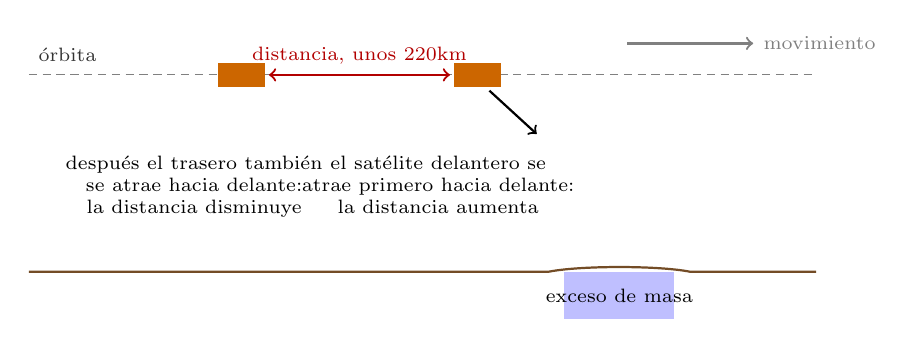
\begin{tikzpicture}[font=\small, x=1cm, y=1cm]
\draw[thick, brown!60!black] (-5,0) -- (1.6,0) .. controls (2.0,0.08) and (3.0,0.08) .. (3.4,0) -- (5,0);
\fill[blue!25] (1.8,0) rectangle (3.2,-0.6);
\node[font=\scriptsize] at (2.5,-0.3) {exceso de masa};
\draw[gray, densely dashed] (-5,2.5) -- (5,2.5);
\node[gray!40!black, font=\scriptsize, anchor=south west] at (-5,2.55) {órbita};
\fill[orange!80!black] (-2.6,2.35) rectangle (-2.0,2.65);
\fill[orange!80!black] (0.4,2.35) rectangle (1.0,2.65);
\draw[<->, red!70!black, thick] (-1.95,2.5) -- (0.35,2.5) node[midway, above, font=\scriptsize] {distancia, unos \qty{220}{km}};
\draw[->, thick] (0.85,2.3) -- (1.45,1.75);
\draw[->, thick, gray] (2.6,2.9) -- (4.2,2.9) node[right, font=\scriptsize] {movimiento};
\node[font=\scriptsize, anchor=north, align=center] at (0.2,1.6) {el satélite delantero se\\atrae primero hacia delante:\\la distancia aumenta};
\node[font=\scriptsize, anchor=north, align=center] at (-2.9,1.6) {después el trasero también\\se atrae hacia delante:\\la distancia disminuye};
\end{tikzpicture}

\par\smallskip{\small El principio del par de satélites (esquemático, no a
escala). Al acercarse a un exceso de masa, el satélite delantero es el primero en sentir su atracción y se acelera hacia delante, con lo que la distancia entre los dos aumenta;
cuando el satélite trasero llega sobre la masa, la distancia vuelve a disminuir. La
velocidad relativa, medida de forma continua,
se invierte para obtener el campo gravitatorio.}
\label{fig:b3:gravity-geodesy:grace}
\end{omfigure}

\begin{omfigure}
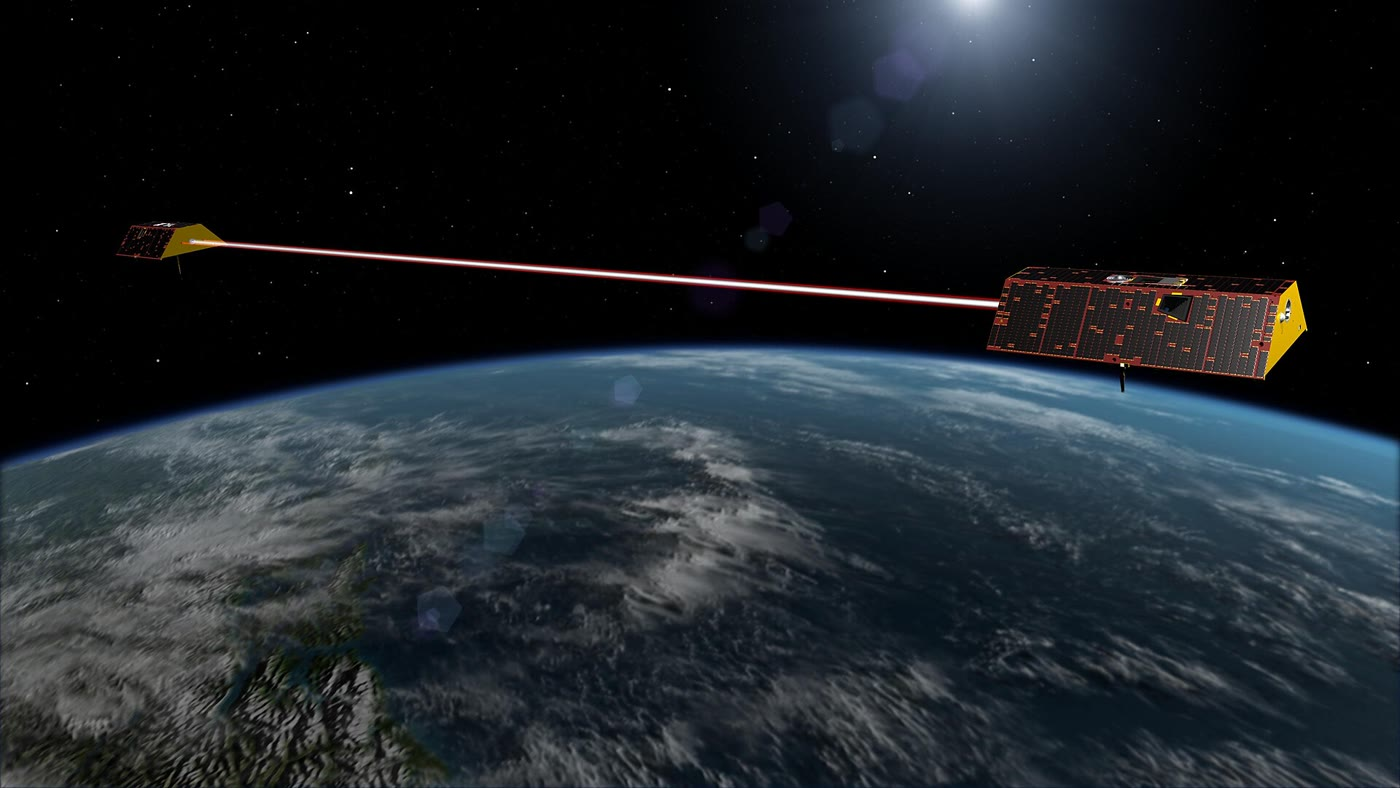
\includegraphics[width=0.66\linewidth]{images/book5/b3-grace-fo-concept.jpg}

\par\smallskip{\small Los dos satélites GRACE Follow-On, vistos por un artista (la
distancia entre ellos está muy reducida). El haz rojo representa el enlace láser
de medida de distancia. NASA/JPL-Caltech, dominio público.}
\label{fig:b3:gravity-geodesy:grace-photo}
\end{omfigure}

\begin{definition}[Altura de agua equivalente]\label{def:b3:gravity-geodesy:ewh}
Un cambio del campo gravitatorio que varía lentamente a distancias mucho mayores
que el espesor de la capa donde se desplazó la masa puede representarse mediante un
cambio de densidad superficial $\sigma$ (\unit{kg.m^{-2}}) sobre una capa delgada en la
superficie terrestre. La \emph{altura de agua equivalente}\index{altura de agua equivalente}
es el espesor de agua dulce con la misma densidad superficial:
\[
  h_w = \frac{\sigma}{\rho_w} .
\]
\end{definition}

Un metro de agua sobre una cuenca de \qty{1e6}{km^2} es \qty{1e15}{kg}, o
\qty{1000}{Gt}. El nivel del mar es la otra cara del balance: \qty{360}{Gt} de hielo
añadido al océano lo eleva unos \qty{1}{mm}.
% ledger: data:b5-imbie
La \omterm{def:b3:gravity-geodesy:satgrav}{gravimetría por satélite}, la altimetría por satélite y el balance de las nevadas frente a
la descarga de hielo miden cada una el balance de masa de los casquetes de hielo; combinadas,
dan la serie que se muestra a continuación.

\begin{omfigure}
\begin{tikzpicture}
\begin{axis}[omrecord, width=0.82\linewidth, height=0.5\linewidth,
  xmin=1992, xmax=2021, ymin=-5600, ymax=600,
  xlabel={año}, ylabel={cambio de masa acumulado (\unit{Gt})},
  xticklabel style={/pgf/number format/1000 sep={}},
  legend pos=south west, legend cell align=left, legend style={font=\scriptsize}]
\addplot[name path=gl, draw=none, forget plot] table[x=year, y=lo] {figdata/out/bachelor-3-ice_mass-greenland.dat};
\addplot[name path=gh, draw=none, forget plot] table[x=year, y=hi] {figdata/out/bachelor-3-ice_mass-greenland.dat};
\addplot[blue!25, forget plot] fill between[of=gl and gh];
\addplot[name path=al, draw=none, forget plot] table[x=year, y=lo] {figdata/out/bachelor-3-ice_mass-antarctica.dat};
\addplot[name path=ah, draw=none, forget plot] table[x=year, y=hi] {figdata/out/bachelor-3-ice_mass-antarctica.dat};
\addplot[red!20, forget plot] fill between[of=al and ah];
\addplot[blue!70!black, thick] table[x=year, y=cum] {figdata/out/bachelor-3-ice_mass-greenland.dat};
\addlegendentry{Groenlandia}
\addplot[red!70!black, thick] table[x=year, y=cum] {figdata/out/bachelor-3-ice_mass-antarctica.dat};
\addlegendentry{Antártida}
\draw[gray, densely dotted] (axis cs:2002.25,-5600) -- (axis cs:2002.25,600);
\draw[gray, densely dotted] (axis cs:2017.5,-5600) -- (axis cs:2017.5,600);
\node[font=\scriptsize, gray!40!black, anchor=north] at (axis cs:2009.9,550) {años GRACE};
\end{axis}
\end{tikzpicture}

\par\smallskip{\small Cambio de masa acumulado de los casquetes de hielo de Groenlandia
y de la Antártida desde 1992, con bandas de una desviación estándar (estimaciones reconciliadas
de IMBIE 2021 a partir de altimetría, gravimetría y el método entrada-salida). A finales
de 2020, Groenlandia había perdido $\num{4890} \pm \qty{460}{Gt}$ y la Antártida
$\num{2670} \pm \qty{530}{Gt}$; los ajustes lineales dan \qty{-176}{Gt.yr^{-1}} y
\qty{-91}{Gt.yr^{-1}} entre 1992 y 2020, y \qty{-246}{Gt.yr^{-1}} y
\qty{-127}{Gt.yr^{-1}} durante los años GRACE.}
\label{fig:b3:gravity-geodesy:ice-mass}
\end{omfigure}

Una anomalía de la gravedad medida en la superficie es una suma de armónicos; a la
altura de un satélite, cada uno se debilita en un factor que depende de su
longitud de onda.

\begin{proposition}[Prolongación ascendente]\label{prop:b3:gravity-geodesy:upward}
Por encima de las masas que la causan, una anomalía de la gravedad que varía a lo largo de la superficie
como $\Delta g_0\cos kx$, con $k = 2\pi/\lambda$, se encuentra a la altura $z$ (su
\emph{prolongación ascendente}\index{prolongación ascendente})
\[
  \Delta g(x, z) = \Delta g_0\,e^{-kz}\cos kx .
\]
\end{proposition}

\begin{proof}
Por encima de las masas, el potencial anómalo, y con él la anomalía, satisface la
ecuación de Laplace $\partial_x^2\Delta g + \partial_z^2\Delta g = 0$. Separando
variables, $\Delta g = Z(z)\cos kx$ con $Z'' = k^2Z$, cuya solución acotada cuando
$z \to \infty$ es $Z = \Delta g_0e^{-kz}$.
\end{proof}

A una altitud de \qty{400}{km}, una anomalía de \qty{1000}{km} de longitud conserva el \qty{8}{\percent}
de su amplitud, y una de \qty{100}{km} de longitud, aproximadamente \num{1e-11} de la suya:
los satélites detectan las longitudes de onda largas, y los estudios en la superficie, las cortas.

\section{Flexión de la litosfera}

El volumen de primer año compensaba una carga de forma local, cada columna flotando sobre sí misma.
Un volcán sobre una placa oceánica no se compensa solo bajo sí mismo: la placa se curva bajo él
en una anchura de cientos de kilómetros, y el fondo marino
que rodea al volcán se hunde en un foso, más allá del cual se eleva en un arco bajo.

\begin{definition}[Flexión litosférica, rigidez a la flexión, espesor elástico efectivo]\label{def:b3:gravity-geodesy:flexure}
La \emph{flexión litosférica}\index{flexión litosférica} es la curvatura de la
litosfera bajo una carga, modelizada como la flexión de una placa elástica delgada
que flota sobre un manto fluido. La resistencia de la placa a la flexión es su
\emph{rigidez a la flexión}\index{rigidez a la flexión}
\[
  D = \frac{ET_e^3}{12(1 - \nu^2)},
\]
y el espesor $T_e$ de la placa elástica uniforme que se curva como la litosfera real es su
\emph{espesor elástico efectivo}\index{espesor elástico efectivo}.
\end{definition}

\begin{theorem}[Flexión de una placa delgada]\label{thm:b3:gravity-geodesy:plate}
Una placa elástica delgada de rigidez $D$, curvada en una dirección por una carga $q(x)$
por unidad de área, deflectada hacia abajo $w(x)$ y flotando sobre un manto de densidad
$\rho_m$, quedando el hueco rellenado con material de densidad $\rho_i$, cumple la
\emph{ecuación de la flexión}\index{ecuación de la flexión}
\[
  D\frac{\mathrm d^4w}{\mathrm dx^4} + (\rho_m - \rho_i)g\,w = q(x) .
\]
\end{theorem}

\begin{proof}
En una placa curvada, las fibras por encima del plano medio se acortan y las de debajo se estiran,
en proporción a la curvatura $w''$; integrando el esfuerzo de flexión
a lo largo del espesor se obtiene el momento flector $M = -Dw''$, con la
rigidez de la definición (la placa no puede dilatarse lateralmente, de ahí el factor
$1 - \nu^2$; los libros de física de tercer año). Una rebanada $\mathrm dx$ de la placa
soporta en sus caras la fuerza cortante $V$ y el momento $M$. Equilibrio vertical:
la carga $q\,\mathrm dx$ hacia abajo y el empuje del manto desplazado
$(\rho_m - \rho_i)gw\,\mathrm dx$ hacia arriba dan $\mathrm dV/\mathrm dx = -q +
(\rho_m - \rho_i)gw$. El equilibrio de momentos da $\mathrm dM/\mathrm dx = V$.
Entonces $-Dw'''' = M'' = V' = -q + (\rho_m - \rho_i)gw$.
\end{proof}

\begin{definition}[Parámetro de flexión, abultamiento periférico]\label{def:b3:gravity-geodesy:alpha}
El \emph{parámetro de flexión}\index{parámetro de flexión} de una placa es la
longitud
\[
  \alpha = \left(\frac{4D}{(\rho_m - \rho_i)g}\right)^{1/4},
\]
que fija la escala horizontal de su flexión. El \emph{abultamiento periférico}\index{abultamiento periférico}
es el arco bajo de flexión ascendente que una placa curvada levanta más allá del foso o
cuenca junto a su carga.
\end{definition}

\begin{proposition}[Carga lineal sobre una placa continua]\label{prop:b3:gravity-geodesy:line}
Una carga lineal $V_0$ por unidad de longitud a lo largo de $x = 0$ deforma la placa en
\[
  w(x) = w_0e^{-|x|/\alpha}\left(\cos\frac{|x|}{\alpha} + \sin\frac{|x|}{\alpha}\right),
  \qquad w_0 = \frac{V_0\alpha^3}{8D} .
\]
La deflexión se anula en $|x| = 3\pi\alpha/4$, el borde del foso; la
cresta del \omterm{def:b3:gravity-geodesy:alpha}{abultamiento periférico} está en $|x| = \pi\alpha$, con altura $w_0e^{-\pi} =
\num{0.0432}\,w_0$. El empuje de toda la deflexión equilibra la carga:
$\int(\rho_m - \rho_i)gw\,\mathrm dx = V_0$.
\end{proposition}

\begin{proof}
Para $x > 0$ la ecuación es $w'''' + 4w/\alpha^4 = 0$; las raíces de
$r^4 = -4/\alpha^4$ son $(\pm1 \pm i)/\alpha$, y las soluciones que se anulan lejos
son $e^{-x/\alpha}(A\cos(x/\alpha) + B\sin(x/\alpha))$. La simetría impone
$w'(0) = 0$, lo que da $A = B = w_0$. Integrando el equilibrio vertical a través
de la carga, la fuerza cortante $V = -Dw'''$ salta en $-V_0$; por simetría
$w'''(0^-) = -w'''(0^+)$, y $w'''(0^+) = 4w_0/\alpha^3$, luego $8Dw_0/\alpha^3 =
V_0$. La deflexión se anula donde $\tan(x/\alpha) =
-1$, por primera vez en $x = 3\pi\alpha/4$; su derivada,
$-(2w_0/\alpha)e^{-x/\alpha}\sin(x/\alpha)$, se anula a continuación en $x = \pi\alpha$.
Por último, $\int_0^\infty e^{-u}(\cos u + \sin u)\,\mathrm du = 1$, así que
$\int w\,\mathrm dx = 2w_0\alpha = V_0\alpha^4/(4D) = V_0/((\rho_m - \rho_i)g)$.
\end{proof}

\begin{proposition}[Placa rota]\label{prop:b3:gravity-geodesy:broken}
Una placa rota en $x = 0$ y empujada hacia abajo en su extremo libre, como en una
fosa oceánica profunda, se deforma según $w = w_0e^{-x/\alpha}\cos(x/\alpha)$ para $x \ge 0$: la
deflexión se anula en $x = \pi\alpha/2$, y la cresta del \omterm{def:b3:gravity-geodesy:alpha}{abultamiento periférico}, el
levantamiento exterior, está en $x = 3\pi\alpha/4$, con altura $w_0e^{-3\pi/4}/\sqrt2 =
\num{0.067}\,w_0$.
\end{proposition}

\begin{proof}
Las mismas soluciones decrecientes, ahora con el extremo libre sin momento,
$w''(0) = 0$, lo que da $B = 0$. El cero está en $\cos(x/\alpha) = 0$; la
derivada $-(w_0/\alpha)e^{-x/\alpha}(\cos + \sin)(x/\alpha)$ se anula en
$x = 3\pi\alpha/4$, donde $w = w_0e^{-3\pi/4}\cos(3\pi/4)$.
\end{proof}

Las distancias son, por tanto, la clave de la resistencia de la placa: si se mide dónde
termina el foso o dónde culmina el abultamiento, se obtiene $\alpha$, después $D$ y luego $T_e$.
Como $T_e$ entra como $\alpha^{4/3}$, una estimación razonable de una distancia da una buena
estimación del espesor.

\begin{omfigure}
\begin{tikzpicture}
\begin{groupplot}[group style={group size=1 by 2, vertical sep=1.5cm},
  width=0.82\linewidth, height=0.36\linewidth, xmin=-400, xmax=400,
  tick label style={font=\scriptsize}, label style={font=\small}, title style={font=\small}]
\nextgroupplot[title={(a) carga lineal: la cordillera de Oru sobre placas de tres espesores},
  ylabel={deflexión (\unit{m})}, ymin=-3000, ymax=700, y filter/.expression={-y},
  legend pos=south east, legend cell align=left, legend style={font=\scriptsize}]
\addplot[red!70!black, thick] table[x=x, y=w10] {figdata/out/bachelor-3-flexure-profiles.dat};
\addlegendentry{$T_e = \qty{10}{km}$}
\addplot[blue!70!black, thick] table[x=x, y=w25] {figdata/out/bachelor-3-flexure-profiles.dat};
\addlegendentry{$T_e = \qty{25}{km}$}
\addplot[green!45!black, thick] table[x=x, y=w40] {figdata/out/bachelor-3-flexure-profiles.dat};
\addlegendentry{$T_e = \qty{40}{km}$}
\draw[gray] (axis cs:-400,0) -- (axis cs:400,0);
\draw[->, blue!70!black] (axis cs:222,330) -- (axis cs:222,90);
\node[font=\scriptsize, blue!70!black, anchor=south] at (axis cs:222,330) {abultamiento periférico, $\pi\alpha$};
\nextgroupplot[title={(b) placa rota en una fosa, $T_e = \qty{25}{km}$},
  xlabel={distancia a la carga o a la fosa (\unit{km})},
  ylabel={deflexión (\unit{m})}, xmin=0, xmax=400, ymin=-1100, ymax=280,
  y filter/.expression={-y}]
\addplot[blue!70!black, thick] table[x=x, y=w] {figdata/out/bachelor-3-flexure-broken.dat};
\draw[gray] (axis cs:0,0) -- (axis cs:400,0);
\draw[->] (axis cs:166.5,200) -- (axis cs:166.5,80);
\node[font=\scriptsize, anchor=west] at (axis cs:170,200) {levantamiento exterior, $3\pi\alpha/4$};
\end{groupplot}
\end{tikzpicture}

\par\smallskip{\small Flexión de una placa elástica (calculada;
$E = \qty{100}{GPa}$, $\nu = 0.25$, manto \qty{3300}{kg.m^{-3}}, agua en el
foso; escala vertical muy exagerada). (a) Bajo la carga de una cresta
volcánica (\qty{4.17e12}{N.m^{-1}}), una placa delgada se hunde profunda y estrechamente; una gruesa,
poco y ampliamente; el \omterm{def:b3:gravity-geodesy:alpha}{abultamiento periférico} se desplaza desde \qty{112}{km} hasta
\qty{316}{km}. (b) Una placa rota en una fosa y empujada hacia abajo \qty{1}{km}:
el levantamiento exterior se eleva \qty{67}{m}, a \qty{167}{km} de la fosa.}
\label{fig:b3:gravity-geodesy:flexure}
\end{omfigure}

\begin{definition}[Compensación isostática regional]\label{def:b3:gravity-geodesy:regional}
La \emph{compensación isostática regional}\index{compensación isostática regional}
es el sostenimiento de una carga por la flotabilidad de una deflexión que se extiende
sobre una región más ancha que la carga, mediante la resistencia a la flexión de la litosfera; en la
compensación de Airy o de Pratt, en cambio, cada columna se compensa por debajo de sí misma.
\end{definition}

La compensación local y la regional equilibran la misma masa total, pero la
distribuyen de forma distinta: bajo una carga estrecha sobre una placa rígida la
raíz es somera y ancha, y la anomalía de la gravedad sobre la carga es fuertemente positiva,
flanqueada por anomalías negativas sobre el foso. Alrededor de las islas de la dorsal de Hawái, los perfiles de gravedad y
sísmicos dan \omterm{def:b3:gravity-geodesy:flexure}{espesores elásticos efectivos} de 17 a \qty{37}{km}, y
de 10 a \qty{20}{km} a lo largo de los montes submarinos más antiguos de la cadena del Emperador,
una diferencia esperable a partir de las edades de los volcanes y de la placa que cargaron;
los valores siguen la profundidad de una isoterma cercana a
\qty{350}{\degreeCelsius} en la placa oceánica en enfriamiento.
% ledger: watts25:te
La misma flexión, bajo el peso de un cinturón montañoso, abre las cuencas de
antepaís del volumen de segundo año, en su capítulo sobre la orogenia alpina.

\begin{omfigure}
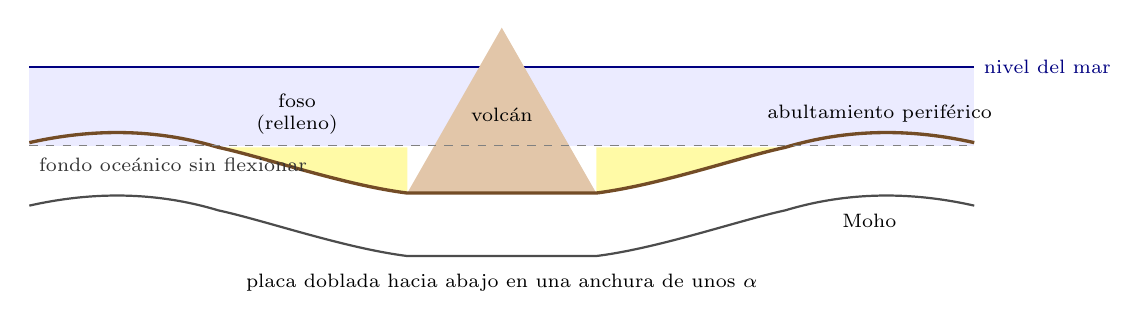
\begin{tikzpicture}[font=\scriptsize, x=1cm, y=1cm]
\fill[blue!8] (-6,0) rectangle (6,-1.0);
\draw[blue!50!black] (-6,0) -- (6,0) node[right] {nivel del mar};
% volcano
\fill[brown!45] (-1.2,-1.6) -- (0,0.5) -- (1.2,-1.6) -- cycle;
% moat infill
\fill[yellow!35] (-1.2,-1.6) .. controls (-2.0,-1.5) and (-3.0,-1.15) .. (-3.6,-1.02) -- (-1.2,-1.02) -- cycle;
\fill[yellow!35] (1.2,-1.6) .. controls (2.0,-1.5) and (3.0,-1.15) .. (3.6,-1.02) -- (1.2,-1.02) -- cycle;
% flexed seafloor (top of crust)
\draw[very thick, brown!60!black] (-6,-0.96) .. controls (-5.2,-0.78) and (-4.4,-0.78) .. (-3.6,-1.02)
  .. controls (-3.0,-1.15) and (-2.0,-1.5) .. (-1.2,-1.6) -- (1.2,-1.6)
  .. controls (2.0,-1.5) and (3.0,-1.15) .. (3.6,-1.02) .. controls (4.4,-0.78) and (5.2,-0.78) .. (6,-0.96);
% Moho, parallel
\draw[thick, gray!60!black] (-6,-1.76) .. controls (-5.2,-1.58) and (-4.4,-1.58) .. (-3.6,-1.82)
  .. controls (-3.0,-1.95) and (-2.0,-2.3) .. (-1.2,-2.4) -- (1.2,-2.4)
  .. controls (2.0,-2.3) and (3.0,-1.95) .. (3.6,-1.82) .. controls (4.4,-1.58) and (5.2,-1.58) .. (6,-1.76);
\node[anchor=west] at (4.2,-1.95) {Moho};
\draw[dashed, gray] (-6,-1.0) -- (6,-1.0);
\node[anchor=north west, gray!40!black] at (-6,-1.03) {fondo oceánico sin flexionar};
\node[anchor=south, align=center] at (-2.6,-0.98) {foso\\(relleno)};
\node[anchor=south] at (4.8,-0.82) {abultamiento periférico};
\node at (0,-0.6) {volcán};
\node[anchor=north] at (0,-2.5) {placa doblada hacia abajo en una anchura de unos $\alpha$};
\end{tikzpicture}

\par\smallskip{\small Una isla volcánica sobre una placa oceánica (corte transversal
esquemático, escala vertical exagerada). La placa se curva bajo el volcán;
la depresión que lo rodea, el foso, se rellena de restos volcánicos y sedimento, y
más allá la placa se eleva en un \omterm{def:b3:gravity-geodesy:alpha}{abultamiento periférico} bajo.}
\label{fig:b3:gravity-geodesy:moat}
\end{omfigure}

\begin{inthefield}[Un estudio de gravedad relativa]
\begin{minipage}[t]{0.55\linewidth}\vspace{0pt}
Un gravímetro absoluto deja caer un espejo de esquina en una cámara de vacío, una
y otra vez, y mide su caída con un interferómetro láser y un reloj atómico;
da la gravedad en una estación, pero es pesado y lento de instalar. El levantamiento
en sí se hace con un gravímetro relativo, una pequeña balanza de resorte que mide
diferencias de gravedad. El geofísico lo nivela sobre una placa base en cada
estación de una línea, lo lee, anota la hora y la altura, y avanza; cada
pocas horas el circuito vuelve a una estación base, de modo que la lenta deriva del
resorte y las mareas de la Tierra sólida puedan medirse y eliminarse. Un receptor de satélite
sobre un poste cercano da la posición y la altura, porque la gravedad
cambia unos \qty{0.3}{\milli\gal} por cada metro de altura.
\end{minipage}\hfill
\begin{minipage}[t]{0.42\linewidth}\vspace{0pt}
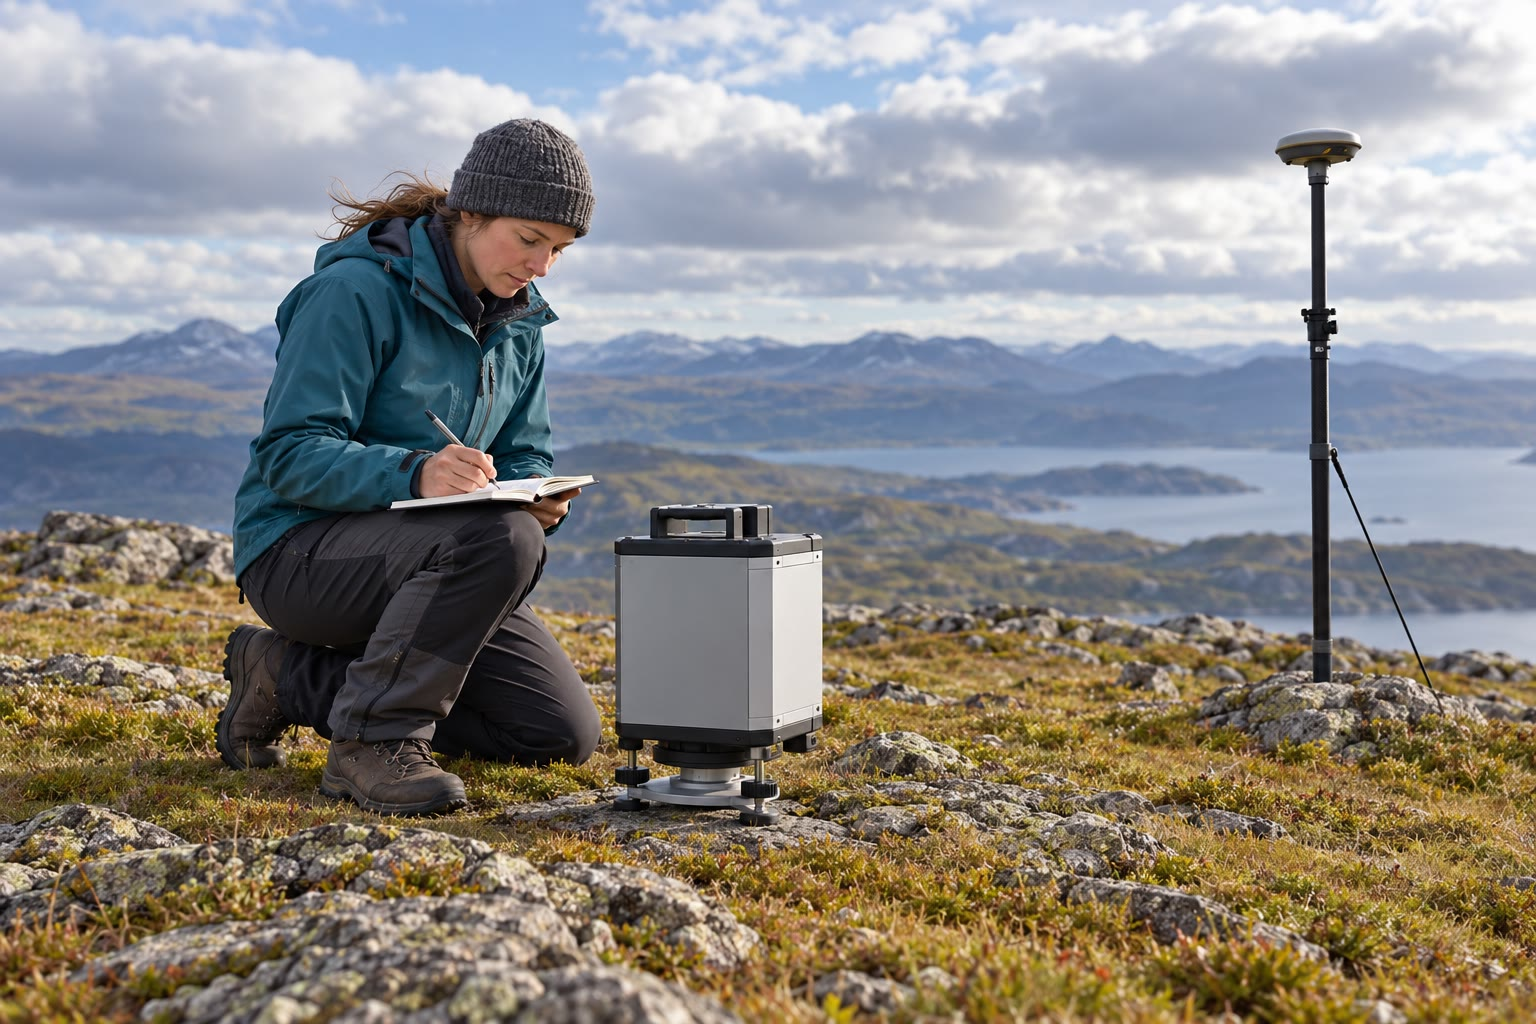
\includegraphics[width=\linewidth]{images/book5/ai/b3-gravimeter.jpg}

{\scriptsize Un gravímetro de campo sobre su base de nivelación, con una antena
de satélite al fondo (ilustración generada por IA).}
\end{minipage}
\end{inthefield}

\section{Ejercicios}

\begin{exercise}[$\star$]\label{exo:b3:gravity-geodesy:1}
A partir de los valores del Sistema Geodésico de Referencia 1980 $a = \qty{6378137}{m}$ y
$f = \num{0.00335281068}$, calcúlese el semieje menor $b$ y $a - b$. Con
$J_2 = \num{1.08263e-3}$ y $m = \num{0.00344979}$, calcúlese el achatamiento que
predice la relación de Clairaut, y compárese.
\end{exercise}

\begin{exercise}[$\star$]\label{exo:b3:gravity-geodesy:2}
En un año seco, una cuenca fluvial de \qty{5.0e5}{km^2} pierde \qty{60}{Gt} de
agua. Calcúlese el cambio de la \omterm{def:b3:gravity-geodesy:ewh}{altura de agua equivalente}.
¿Cuánto subiría el nivel del mar por la misma masa, tomando \qty{360}{Gt} por milímetro?
\end{exercise}

\begin{exercise}[$\star$]\label{exo:b3:gravity-geodesy:3}
Con la serie $\gamma = 9.780327(1 + 0.0053024\sin^2\varphi -
0.0000058\sin^22\varphi)$ \unit{m.s^{-2}}, calcúlese la gravedad normal en el
ecuador, a \ang{45} y en los polos. Exprésese la diferencia entre el polo
y el ecuador en miligales.
\end{exercise}

\begin{exercise}[$\star$]\label{exo:b3:gravity-geodesy:4}
Calcúlese la \omterm{def:b3:gravity-geodesy:flexure}{rigidez a la flexión} y el \omterm{def:b3:gravity-geodesy:alpha}{parámetro de flexión} de placas oceánicas
con $T_e = \qty{10}{km}$ y $T_e = \qty{30}{km}$ ($E = \qty{100}{GPa}$,
$\nu = 0.25$, $\rho_m - \rho_w = \qty{2270}{kg.m^{-3}}$, $g =
\qty{9.81}{m.s^{-2}}$).
¿Dónde están el borde del foso y el \omterm{def:b3:gravity-geodesy:alpha}{abultamiento periférico} bajo una carga lineal?
\end{exercise}

\begin{exercise}[$\star\star$]\label{exo:b3:gravity-geodesy:5}
(a) Para una altura del geoide de $+\qty{50}{m}$: calcúlese el potencial perturbador allí,
tomando $\gamma = \qty{9.80}{m.s^{-2}}$. (b) Sobre \qty{100}{km} el geoide se eleva
\qty{10}{m}. ¿En qué ángulo difiere allí la plomada de la normal al
elipsoide? Exprésese en segundos de arco.
\end{exercise}

\begin{exercise}[$\star\star$]\label{exo:b3:gravity-geodesy:6}
A partir de $J_2 = \num{1.08263e-3}$ y del factor de momento de inercia
$C/(Ma^2) = \num{0.3308}$, calcúlese la elipticidad dinámica $H = (C - A)/C$ y
$1/H$. ¿Cuál de los dos números cambiaría en una Tierra homogénea con el mismo $J_2$?
\end{exercise}

\begin{exercise}[$\star\star$]\label{exo:b3:gravity-geodesy:7}
Un satélite describe una órbita circular a \qty{500}{km} sobre el radio ecuatorial
($a = \qty{6378.137}{km}$, $GM = \qty{3.986005e14}{m^3.s^{-2}}$), con una inclinación de
\ang{89}. Calcúlese su período y la velocidad de precesión nodal en grados por día.
¿Por qué las misiones de gravedad eligen órbitas casi polares?
\end{exercise}

\begin{exercise}[$\star\star$]\label{exo:b3:gravity-geodesy:8}
Dos anomalías de \qty{10}{\milli\gal} en la superficie tienen longitudes de onda de
\qty{100}{km} y \qty{1000}{km}. Calcúlense sus amplitudes a \qty{500}{km}
de altitud.
\end{exercise}

\begin{exercise}[$\star\star$]\label{exo:b3:gravity-geodesy:9}
Hacia el océano desde una fosa, la cresta del abultamiento externo se sitúa a \qty{120}{km} del
eje de la fosa. Tomando el modelo de placa rota con agua sobre la placa, calcúlense
$\alpha$, $D$ y $T_e$, y la distancia a la que la placa cruza su
nivel sin flexionar.
\end{exercise}

\begin{exercise}[$\star\star\star$]\label{exo:b3:gravity-geodesy:10}
(a) Compruébese que $w = w_0e^{-u}(\cos u + \sin u)$, $u = x/\alpha$, satisface
$Dw'''' + (\rho_m - \rho_i)gw = 0$ para $x > 0$, con $\alpha$ tal como se ha definido.
(b) Muéstrese que el momento flector $-Dw''$ es máximo bajo la carga y cambia
de signo en $x = \pi\alpha/4$. (c) ¿Dónde es más probable que la placa se agriete en su
superficie superior, y por qué?
\end{exercise}

\begin{exercise}[$\star\star\star$]\label{exo:b3:gravity-geodesy:11}
Con $m = \num{0.00344979}$ y $C/(Ma^2) = \num{0.3308}$, inviértase la
relación de Darwin--Radau para el achatamiento hidrostático. Compárese con
$f = \num{0.00335281}$: calcúlense la diferencia y el exceso de altura del
ecuador sobre la forma hidrostática. ¿Qué dice esto sobre el manto?
\end{exercise}

\begin{exercise}[$\star\star\star$]\label{exo:b3:gravity-geodesy:12}
Un satélite en una órbita circular a \qty{700}{km} de altura debe mantener la misma
orientación respecto al Sol durante todo el año: su nodo debe avanzar \ang{360} en
un año trópico de \num{365.242}~días. Calcúlese la inclinación necesaria.
\end{exercise}

\section{Problema: el foso alrededor de la cresta de Oru}

\begin{problem}[{Problema de fin de semana --- la figura de la Tierra, una carga volcánica,
su foso de flexión y lo que ven de él los satélites}]
\label{pb:b3:gravity-geodesy:1}
% values: calc/ch03.py; GRS80 (geod5:grs80-*), earth:MoI; flexure.py
Oru es una cresta volcánica inventada en un océano: una cadena recta de volcanes coalescentes
de \qty{400}{km} de longitud, construida sobre litosfera oceánica antigua. Su
sección transversal se toma como un triángulo de \qty{80}{km} de ancho en la base y
\qty{6}{km} de altura, de densidad \qty{2800}{kg.m^{-3}}, apoyado sobre un fondo marino
\qty{5}{km} de profundidad. Manto \qty{3300}{kg.m^{-3}}, agua de mar
\qty{1030}{kg.m^{-3}}, $E = \qty{100}{GPa}$, $\nu = 0.25$, $g =
\qty{9.81}{m.s^{-2}}$, $G = \qty{6.674e-11}{m^3.kg^{-1}.s^{-2}}$.

\medskip
\noindent\textbf{Parte I --- La forma de la Tierra.} Utilícese el Sistema Geodésico
de Referencia de 1980: $a = \qty{6378137}{m}$, $b = \qty{6356752.3}{m}$,
$GM = \qty{3.986005e14}{m^3.s^{-2}}$, $J_2 = \num{1.08263e-3}$,
$\omega = \qty{7.292115e-5}{rad.s^{-1}}$, $f = \num{0.00335281}$; y
$C/(Ma^2) = \num{0.3308}$.
\begin{enumerate}
  \item Calcúlese $m = \omega^2a^2b/(GM)$.
  \item Calcúlese el achatamiento que da la relación de Clairaut a partir de $J_2$ y
        $m$, y su inverso.
  \item Calcúlese el achatamiento hidrostático a partir de la relación de Darwin--Radau, y
        su inverso.
  \item Compárense ambos con el achatamiento observado. ¿En cuántos metros se eleva el
        ecuador por encima de la figura hidrostática?
  \item Calcúlese la elipticidad dinámica $H = (C - A)/C$.
\end{enumerate}

\noindent\textbf{Parte II --- La carga.}
\begin{enumerate}[resume]
  \item Calcúlese el área de la sección transversal de la cresta.
  \item Calcúlese la carga lineal $V_0$, considerando toda la cresta sumergida, de modo
        que pese $(\rho_v - \rho_w)g$ por unidad de volumen.
  \item Si la cresta estuviera compensada localmente, a la manera de Airy, por una raíz de
        su propia roca en el manto, ¿a qué profundidad estaría la raíz bajo la
        cresta?
  \item Con compensación local, la raíz terminaría al pie de la cresta,
        a \qty{40}{km} de su eje. La batimetría muestra un foso que se extiende hasta
        \qty{165}{km}. ¿Qué indica esto?
\end{enumerate}

\noindent\textbf{Parte III --- El foso de flexión.} El foso está lleno de agua
($\rho_i = \rho_w$). Un perfil sísmico transversal a la cresta sitúa el techo de la
corteza oceánica de nuevo a su profundidad regional a \qty{165}{km} del eje, y la
cresta del \omterm{def:b3:gravity-geodesy:alpha}{abultamiento periférico} a \qty{220}{km} del eje.
\begin{enumerate}[resume]
  \item Calcúlese el \omterm{def:b3:gravity-geodesy:alpha}{parámetro de flexión} a partir del borde del foso.
  \item Calcúlese de nuevo a partir del \omterm{def:b3:gravity-geodesy:alpha}{abultamiento periférico}. ¿Son coherentes los dos valores?
  \item Tomando $\alpha = \qty{70.0}{km}$, calcúlese la \omterm{def:b3:gravity-geodesy:flexure}{rigidez a la flexión}.
  \item Calcúlese el \omterm{def:b3:gravity-geodesy:flexure}{espesor elástico efectivo}.
  \item Tomando $V_0 = \qty{4.17e12}{N.m^{-1}}$ y $D$ redondeado a tres
        cifras, calcúlese la deflexión bajo el eje.
  \item Calcúlese la altura del \omterm{def:b3:gravity-geodesy:alpha}{abultamiento periférico}.
  \item Compruébese que la flotabilidad de toda la deflexión, $2w_0\alpha(\rho_m -
        \rho_w)g$, equilibra $V_0$.
  \item Compárese $T_e$ con los valores hallados a lo largo de la dorsal hawaiana, de 17 a
        \qty{37}{km}. Compárese la deflexión bajo el eje con la raíz de Airy
        de la pregunta 8.
\end{enumerate}

\noindent\textbf{Parte IV --- La gravedad sobre el foso.} Tómese un armónico de la
flexión, de longitud de onda $2\pi\alpha$ y amplitud $W = \qty{500}{m}$, que deforma
tanto el fondo marino (corteza de \qty{2900}{kg.m^{-3}} bajo agua, a \qty{5}{km} por debajo del
nivel del mar) como el Moho (manto bajo la corteza, a \qty{12}{km} por debajo del nivel del mar). Una
lámina delgada de densidad superficial $\sigma$ produce la anomalía $2\pi G\sigma$
justo encima de ella.
\begin{enumerate}[resume]
  \item Calcúlese la longitud de onda y el número de onda $k$ del armónico.
  \item Calcúlese la amplitud de la anomalía al nivel del mar debida al fondo marino deformado,
        mediante \omterm{prop:b3:gravity-geodesy:upward}{prolongación ascendente} desde \qty{5}{km} de profundidad.
  \item Calcúlese la del Moho deformado, y la total.
  \item Calcúlese el total a la altitud de un satélite, a \qty{400}{km} sobre el nivel del
        mar.
  \item ¿En qué factor se debilita, a esa altitud, un armónico de longitud de onda \qty{80}{km}, la anchura de
        la cresta? ¿Qué puede resolver el satélite?
  \item ¿A qué grado de armónicos esféricos $n \approx 2\pi R/\lambda$ corresponde el
        armónico de la pregunta 18 ($R = \qty{6371}{km}$)?
  \item Indíquese el \omterm{def:b3:gravity-geodesy:flexure}{espesor elástico efectivo} de la placa bajo la cresta de
        Oru.
\end{enumerate}
\end{problem}
